\chapter{Techniques d'imagerie par ultrasons}


 L'objectif de ce chapitre est de présenter les principales méthodes multi-éléments utilisées pour l'imagerie ultrasonore. Les transducteurs multi-éléments sont d'abord utilisés dans les années 70 pour l'imagerie médicale et sont aujourd'hui répandus en contrôle de pièces industriels.\\

Chaque élément piézoélectrique d'un transducteur peut être utilisé en émission puis en réception. Ces éléments étant pilotables indépendamment, il est possible d'appliquer une loi de retard permettant d'orienter le front d'onde source ou de focaliser le faisceau excitateur. Cela permet notamment d'améliorer le rapport signal sur bruit et peut représenter un gain de temps car le balayage d'une pièce à inspecter peut être réalisé sans déplacement du transducteur, par simple focalisation du faisceau.\\

En réception de l'onde sonore, ces transducteurs permettent de réaliser de la formation de voie, dont on distingue trois principaux types de méthodes : 
\begin{itemize}
	\item les méthodes par retard et sommation des signaux,
	\item les méthodes dites "haute résolution",
	\item les méthodes basées sur un problème d'optimisation.
\end{itemize} 

On décrit ici le principe de ces méthodes après avoir présenté les différents modes de représentation des données temporelles.




\section{Représentation des données temporelles}

Lorsque l'onde est perturbée par un changement des propriétés élastiques de son support, il est possible de l'observer directement sur les signaux temporels mesurés. Pour cela, différents modes de représentation sont utilisés. Les échographies peuvent être représentées en un point d'observation (Ascan), sur une ligne de balayage (Bscan) équivalent à une coupe transversale de la pièce,  sur un plan de balayage (Cscan) donnant un vue de surface et ne permettant pas une localisation en profondeur d'un réflecteur. La figure~\ref{scan} (extraite de \cite{bannouf}) montre le type d'images obtenues d'une pièce perforée, pour ces trois modes de représentation des données. \\
 
Ce type d'analyse peut être réalisé avec des transducteurs mono-éléments. L'obtention d'une image 2D nécessite alors un balayage sur l'ensemble d'une surface de la pièce à contrôler. \\

%\begin{figure}[!h]
%	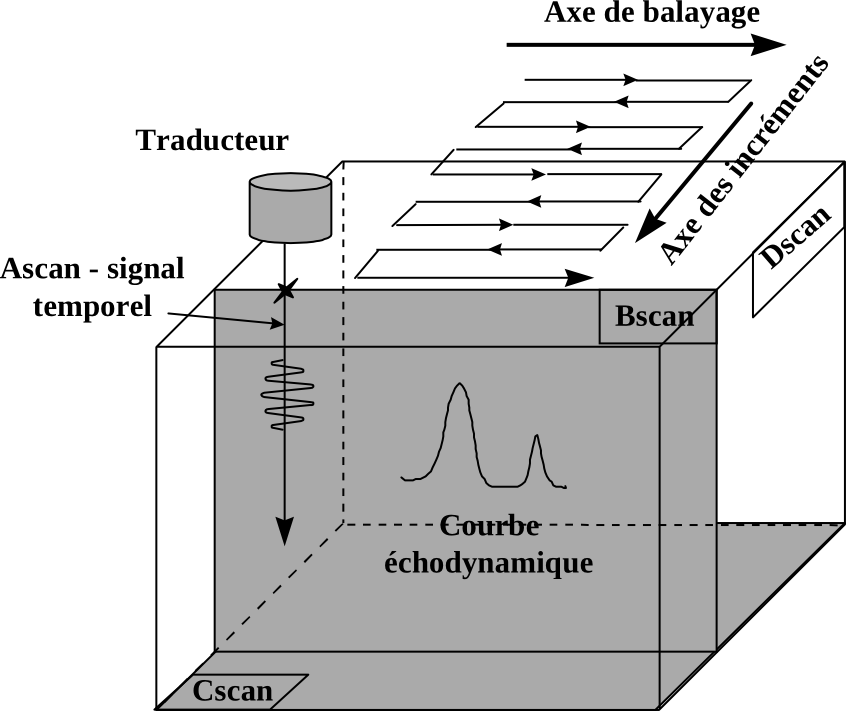
\includegraphics[scale=0.7]{img/scan.png}
%	\caption{\label{scan} Schéma des différents modes de représentation des signaux temporels (extrait de \cite{chassignole}).}
%\end{figure} 

\begin{figure}
	\centering
	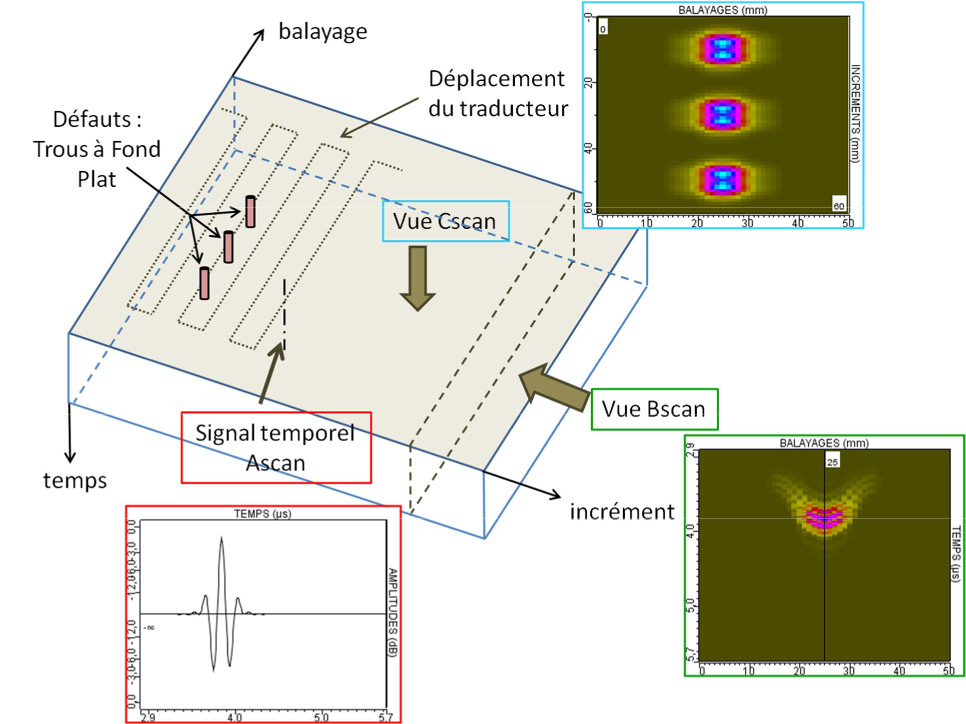
\includegraphics[scale=0.7]{img/scan2.png}
	\caption{\label{scan} Schéma des différents modes de représentation des signaux temporels (extrait de \cite{bannouf}). Le Ascan représente l'amplitude du signal en fonction du temps (en bas à gauche). L'abscisse du Bscan (en bas à droite) donne le balayage, ses ordonnée est le temps et l'échelle de couleurs donne l'amplitude du signal temporel. En haut à droite, le Cscan a pour abscisse l'axe de balayage et en ordonnée les incréments, tandis que l'échelle de couleurs donne l'amplitude du maximum de chaque signal temporel.}
\end{figure}

Il existe une autre représentation, le Sscan, qui ne peut être réalisé qu'avec des transducteurs multi-éléments : il correspond a un ensemble de Ascans réalisés sans déplacement du transducteur mais en appliquant une loi de retard aux éléments permettant de réaliser un balayage du point focal. Le Sscan permet donc d'imager des pièces partiellement accessible, et augmente la probabilité de repérer un défaut en offrant plusieurs angles d'auscultation.\\

Cependant, la localisation dans la pièce des réflecteurs à l'origine des différents échos visibles sur les signaux temporels mesurés n'est possible que si la vitesse de propagation des ondes est connue. Les Bsans dits "vrais" sont des Bscans sur lesquels des corrections des temps de vol liées à la vitesse ou à l'angle d'incidence du faisceau sont appliquées.


\section{Méthodes par retard et sommation des signaux}
Les données temporelles acquises peuvent aussi être traitées de manière à obtenir une représentation spatiale des propriétés de la pièce. Si la vitesse du milieu de propagation est connue, une analyse des temps de vol des échos permet en effet d'établir une carte des vitesses de propagation du milieu. \\

Il est aussi possible de sommer un ensemble de Ascans de façon cohérente, permettant ainsi de reproduire une focalisation en tous points de la zone à inspecter. C'est ce que propose la méthode Synthetic Aperture Focusing Technique \citep{doctor_saft} à partir des signaux recueillis par un mono-élément. Ce procédé est généralisé à un ensemble de capteurs et d'émetteurs dans la méthode Total Focusing Method \citep{holmes_tfm}. 

L'intensité $I$ de l'image obtenue au point de coordonnées $\bm{r}$ est alors donnée par la relation suivante : 

\begin{equation}
	I(\bm{r})= \displaystyle\sum_{r} \displaystyle\sum_{e} s_{r,e}\left( T_{\bm{r}\bm{r}_{r}+T_{\bm{r}\bm{r}_{e}}} \right) \text{,}	
\end{equation}
avec $s_{r,e}$ les signaux temporels pour chaque couple émetteur-récepteur. $T_{\bm{r}\bm{r}_{r}}$ et $T_{\bm{r}\bm{r}_{e}}$ sont les temps de vol pour aller du point d'observation $\bm{r}$ au point de réception $\bm{r}_{r} $ et d'émission $\bm{r}_{e}$. Dans le cas d'un milieu de vitesse homogène $c$, cette expression peut donc se réduire à :

\begin{equation}
	I(\bm{r})= \displaystyle\sum_{r} \displaystyle\sum_{e} s_{r,e}\left( \frac{|\bm{r} - \bm{r}_r| + |\bm{r} - \bm{r}_t|}{c}\right) \text{,}
\end{equation}

Cette focalisation permet donc de couvrir l'ensemble du volume de la pièce car tous les angles peuvent être balayés, indépendamment de l'ouverture du capteur, ce qui permet une meilleure résolution que celle obtenue avec des Bscans.\\






\section{Méthodes haute résolution}


Des méthodes de localisation de sources dites "hautes résolutions" exploitent l'ensemble des covariances des signaux temporels. Les méthodes telles que MUltiple Signal Classification \citep{schmidt} et Capon \citep{capon} proposent une décomposition en valeurs propres de cette matrice de covariance afin d'en extraire deux sous-espaces distincts, l'un associé au signal et l'autre au bruit, diminuant ainsi la contribution énergétique du bruit. \\

La méthode de Décomposition de l'Opérateur de Retournement Temporel \citep{prada_dort} propose, de la même façon, d'interpréter l'opérateur de retournement temporel comme une matrice de covariance et de la décomposer. Cette dernière méthode est particulièrement adaptée aux milieux hétérogènes et/ou à géométrie complexe , car sa résolution est améliorée si le signal mesuré a été mulitplement réfléchi. En effet, le retournement temporel permet une focalisation de l'énergie au niveau d'un point source et cette focalisation est d'autant plus précise que le nombre de sources images est important. \\
  

Tout comme pour les méthodes de formation de voies classiques, il est nécessaire de connaître les propriétés élastiques du milieu de propagation pour pouvoir localiser précisément les réflecteurs.\\

%(billette de titane, par exemple https://www.institut-langevin.espci.fr/IMG/pdf/jasakerbrat-2002.pdf)
%(plaque mince : ondes de lamb https://www.institut-langevin.espci.fr/IMG/pdf/JASAlamb-1998.pdf)

\section{Problème d'optimisation}

L'objectif de ces méthodes est de résoudre un problème inverse en minimisant une fonction coût traduisant l'écart entre les données observées issu du milieu recherché et les données calculées à partir d'un modèle courant \citep{tarantola_book}. Le milieu courant correspond à une évolution d'un modèle initial vers un milieu que l'on identifie comme final suivant le critère de convergence de l'optimisation.\\


Le modèle est décrit par un nombre fini de paramètres $\bm{m}$ qui sont liés à des observables $\bm{d}_{obs}$ par l'intermédiaire de lois physiques $\bm{g}$. La résolution du problème inverse consiste donc à trouver les paramètres $\bm{m}$ qui interprètent le mieux les données observées par les données calculées $\bm{d}_{cal}(\bm{m})$ (cf schéma de la figure~\ref{pb_inv}). 

\begin{figure}[!h]
	\centering
	\begin{tikzpicture}
		\node (param) [draw=black, align=center] at (0,0) {Paramètres initiaux \\ $\bm{m}_{0}$};
		\node (dir) [below=1cm of param , draw=black,align=center] {Problème direct \\ $\bm{g}(\bm{m})$};
		\path[->, thick,shorten <=2pt,shorten >=2pt] (param) edge (dir);
		\node (fc) [draw=black,right=2cm of dir, align=center] {Fonction de coût \\ $\text{écart}\hspace{-1mm}\left(\bm{d}_{obs}, \bm{d}_{cal}(\bm{m})\right)$};
		\path[->, thick,shorten <=2pt,shorten >=2pt] (dir) edge (fc);
		\node (m) [draw=black, below right= and -0.5cm of dir, align=center] {Problème inverse \\$\bm{m}+\Delta\bm{m}$};
		\path[->, thick,shorten <=2pt,shorten >=2pt] (fc) edge (m);
		\path[->, thick,shorten <=2pt,shorten >=2pt] (m) edge (dir);
	\end{tikzpicture} 
	\caption{\label{pb_inv} Schéma de résolution d'un problème d'optimisation. Le modèle courant décrit par les paramètres $\bm{m}$ est mis à jour tant que la fonction de coût n'a pas atteint le minimum donné par le critère de convergence.}
\end{figure}

Ces problèmes sont, en général, non-linéaires, car les observables ne dépendent pas linéairement des paramètres du modèle, ce que l'on note $\bm{d}_{obs}=\bm{g}(\bm{m})$. De plus, le problème est mal posé si ce système d'équation n'est pas de rang plein et la solution n'est alors pas unique.

\subsection{Résolution du problème direct}

Le problème direct peut être résolu soit par des méthodes semi-analytiques (représentation intégrale, méthodes modales,\ldots) soit par des méthodes numériques. Parmi les méthodes numériques les plus usitées figurent les méthodes de différences finies (\citealp{virieux_86}, à l'ordre 2 et \citealp{levander}, à l'ordre 4) populaires par leur simplicité de formulation et d'implémentation et les méthodes des éléments finis (Galerkin discontinu par exemple : \citealp{brossier_these}) ou volumes finis \citep{brossier_2008} qui facilitent l'utilisation des maillages non-structurés. On peut aussi citer la méthode asymptotique des lancers de rayons \citep{virieux_ray} qui favorise les calculs performants et facilite l'interprétation physique des résultats, mais qui ne permet pas un contrôle précis de l'échantillonnage.

\subsection{Résolution du problème inverse}
Si le problème direct possède une solution unique, le problème inverse peut conduire à plusieurs solutions.
Lorsque le nombre de paramètres est grand, le problème inverse ne peut pas être résolu par une recherche exhaustive dans l'espace des solutions. La recherche de solution peut donc se faire par des méthodes semi-globales ou locales, dont quelques unes sont décrites ci-après.\\

\subsubsection{Les méthodes semi-globales}
Les méthodes semi-globales consistent à parcourir l'espace des solutions avec une approche statistiques. Les plus connues sont les améliorations de celle de Monte Carlo comme le recuit simulé \citep{tarantola_book, sen} ou  la méthode de Monte-Carlo par chaînes de Markov \citep{zhang}, ainsi que les algorithmes génétiques \citep{stoffa}. Elles permettent d'obtenir une solution avec peu d'\emph{a priori} sur le modèle initial, mais avec une convergence lente.\\

\subsubsection{Les méthodes locales}
Lorsque que le modèle initial peu être construit avec suffisamment d'informations pour que le problème se situe proche du minimum global recherché, des méthodes d'optimisation moins coûteuses sont envisageables. Ces méthodes se basent sur l'estimation du gradient et du hessien de la fonction coût pour estimer sa plus forte pente et sa courbure.\\

La méthode de recherche linéarisée la plus simple est celle du gradient (ou algorithme de la plus forte pente), qui permet d'effectuer au point courant, un pas de descente dans la direction opposée au gradient. Les directions de descentes successives sont alors orthogonales, ce qui ne permet pas une convergence très rapide. \\
La méthode du gradient conjugué propose de combiner les directions de descente des itérations précédentes de façon à accélérer la convergence. Cette méthode populaire est celle utilisée par Mora et Tarantola dans les années 80 \citep{tarantola_84, mora_87a, mora_87b}. Le hessien n'est pas calculé, mais cette méthode nécessite le calcul de deux problèmes directs supplémentaires. \\

Les méthodes de Newton et de Gauss-Newton utilisent un calcul du hessien (complet pour la première, approximé pour la seconde). Le hessien est difficile à calculer car sa complexité est celle du gradient au carré, mais il permet une convergence plus rapide qu'avec la méthode du gradient conjugué \citep{pratt_98}.\\

Enfin, le hessien peut également être estimé à partir des gradients des itérations précédentes, par la méthode quasi-Newton \citep{nocedal}, avec l'algorithme BFGS (Broyden, Fletcher, Goldfarb, Shanno), par exemple. Cet algorithme ayant un gros coût de stockage, il existe des versions allégées fournissant une estimation du hessien à partir du stockage de quelques itérations seulement (L-BFGS). 
\subsection{Cartographie ou contour}
Comme le souligne \cite{mat_ac}, le problème inverse peut être résolu suivant deux approches : 
\begin{itemize}
	\item un formalisme en intégrales de contour où les paramètres reconstruits sont ceux décrivant ces contours. Cela revient donc à déformer ces contours, fonction d'une structure topologique du milieu. Le gradient, donné par la dérivée de la fonction coût par rapport à la topologie, indique donc directement la position d'un défaut à fort contraste. \cite{dominguez} et \cite{rodriguez} utilisent par exemple cette approche pour des applications en contrôle non destructif. Cette approche permet par exemple d'imager des défauts liés à une absence de matière (porosité, fissure, délaminage,\ldots) mais ne prend pas en compte les variations de contraste plus faible (anisotropie de la soudure, inclusion, corps étranger,\ldots).
	\item une reconstruction pixelisée d'un ensemble de paramètres. C'est l'approche explorée dans ce rapport et qui est décrite au chapitre~\ref{fwi}.
\end{itemize}


%-mais aussi : diffraction tomograhy, filtered backpropagation... : techniques basées sur une version linéarisée des équations, born approx par ex, kirchhoff approx


\section{Spécificités de l'imagerie de soudure}

Les méthodes basées sur des analyses de temps de vol, qui nécessitent de connaître la vitesse de propagation de l'onde sont peu adaptées à l'imagerie de soudure. En effet, comme le montrent les macrographies de la figure~\ref{soudure}, les passes multiples et la cristallisation inhomogène rendent la soudure fortement anisotrope \citep{chassignole}. Cette anisotropie varie d'une soudure à une autre puisqu'elle dépend des paramètres de soudage. En conséquence, cette anisotropie engendre une courbure voire une division du faisceau ultrasonore (cf figure \ref{echos}). Les scans sont alors difficiles à analyser et les méthodes par retard et sommation ne permettent pas de relocaliser précisément un réflecteur et les images obtenues sont très sujettes aux artefacts provenant d'échos mal interprétés.

\begin{figure}[!h]
	\hspace{-2cm}
    \centering
    \begin{subfigure}[c]{0.25\textwidth}
    	\centering
        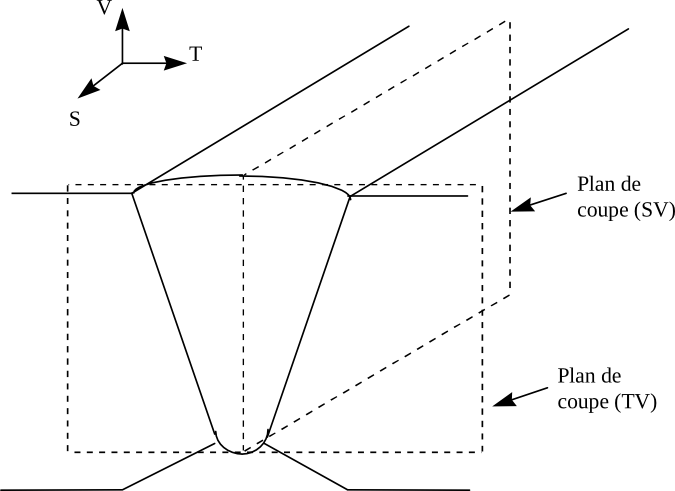
\includegraphics[height=3.5cm]{./img/soudure3.png}
        \vspace{0.03cm}
        \caption{ Définition des plans de coupe.}
    \end{subfigure}
    \hspace{1cm}
    \begin{subfigure}[c]{0.25\textwidth}
    	\centering
        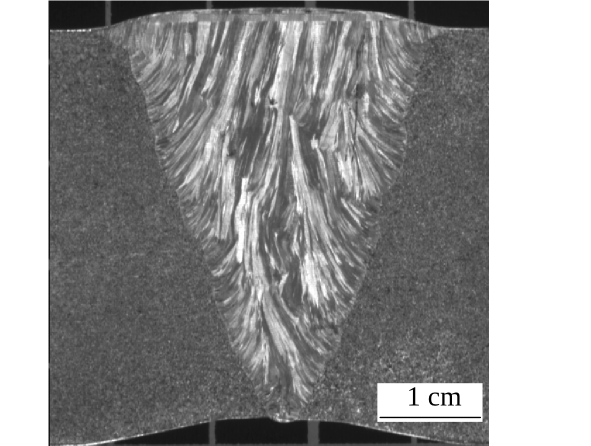
\includegraphics[height=4cm]{./img/soudure1.png}
        \caption{ Coupe dans le plan (TV).}
    \end{subfigure}
        \hspace{1.5cm}
    \begin{subfigure}[c]{0.25\textwidth}
    	\centering
		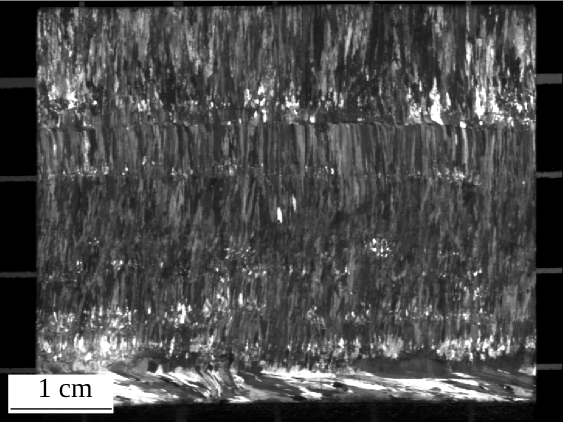
\includegraphics[height=4cm]{./img/soudure2.png}
        \caption{Coupe dans le plan (SV).}
    \end{subfigure}
    \caption{ Macrographie d'une soudure industrielle en acier austénitique  : illustration de la forte anisotropie obtenue par la cristallisation et les passes multiples (images extraites de \cite{chassignole} ). \label{soudure}}
\end{figure}

\begin{figure}[!h]
    \centering
    \begin{subfigure}[c]{0.3\textwidth}
    	\centering
        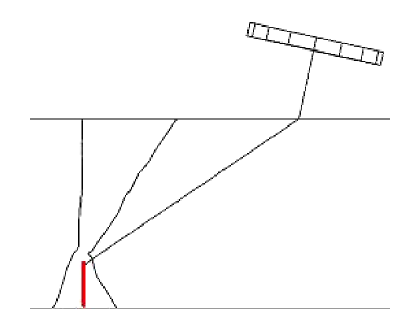
\includegraphics[height=4cm]{img/chassignole_echos_config.png}
        \caption{ Configuration de mesure. En rouge : encoche de 15~mm de haut dans la soudure.}
    \end{subfigure}
    \hspace{1cm}
    \begin{subfigure}[c]{0.3\textwidth}
    	\centering
        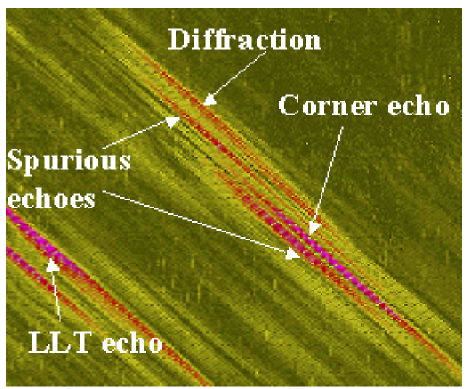
\includegraphics[height=4cm]{img/chassignole_echos.png}
        \caption{Bscan}
    \end{subfigure}
    \caption{Illustration de la perturbation du faisceau ultrasonore dans une sourdure comportant une encoche.  LLT echo : Réflexion de l'onde longitudinale (L) sur le bord de soudure puis réflexion de cette onde L sur l'encoche avec conversion en mode transverse (T).Images extraites de \cite{chassignole_beam}  }\label{echos}
\end{figure}

De manière générale, les méthodes nécessitant une bonne connaissance \emph{a priori} du matériau ne sont pas adaptées à l'imagerie de soudure. Tenter de reconstruire les paramètres élastiques de la soudure par une résolution de problème inverse semble être une approche plus appropriée et intéressante à explorer.


%hohne\_2012 pour images SAFT


%gardahaut pour porpagation de rai CIVA

%Born : linéarise le pb ? (pour faible contraste, adapté au cnd ?) brossier these dit que c'est pas linéarisé et qu'on a donc le champ d'onde complet

%+acoustique non-linéaire : Nonlinear signal processing for ultrasonic imaging of material complexity (dos santos) par ex
